\documentclass{article}
\usepackage{graphicx}
\usepackage[center]{caption}
% If you're new to LaTeX, here's some short tutorials:
% https://www.overleaf.com/learn/latex/Learn_LaTeX_in_30_minutes
% https://en.wikibooks.org/wiki/LaTeX/Basics

% Formatting
\usepackage[utf8]{inputenc}
\usepackage[margin=1in]{geometry}
\usepackage[titletoc,title]{appendix}

% Math
% https://www.overleaf.com/learn/latex/Mathematical_expressions
% https://en.wikibooks.org/wiki/LaTeX/Mathematics
\usepackage{amsmath,amsfonts,amssymb,mathtools}
\usepackage{bm}
\usepackage{siunitx}

% Images
% https://www.overleaf.com/learn/latex/Inserting_Images
% https://en.wikibooks.org/wiki/LaTeX/Floats,_Figures_and_Captions
\usepackage{graphicx,float}

% Tables
% https://www.overleaf.com/learn/latex/Tables
% https://en.wikibooks.org/wiki/LaTeX/Tables

% Algorithms
% https://www.overleaf.com/learn/latex/algorithms
% https://en.wikibooks.org/wiki/LaTeX/Algorithms
\usepackage[ruled,vlined]{algorithm2e}
\usepackage{algorithmic}

% Code syntax highlighting
% https://www.overleaf.com/learn/latex/Code_Highlighting_with_minted
\usepackage{minted}
\usemintedstyle{borland}

% References
% https://www.overleaf.com/learn/latex/Bibliography_management_in_LaTeX
% https://en.wikibooks.org/wiki/LaTeX/Bibliography_Management
\usepackage{biblatex}
\addbibresource{references.bib}

\DeclareMathOperator{\taninv}{tan\,inverse}

% Title content
\title{ENPM 673 Project 1}
\author{Arjun Srinivasan Ambalam, Praveen Menaka Sekar, Arun Kumar Dhandayuthabani}
\begin{document}

\maketitle

% Introduction and Overview
\section{Introduction}
The project focuses on detecting a custom AR Tag (a form of fiducial marker), that is used for obtaining a point of reference in the real world, such as in augmented reality applications. The two aspects to using an AR Tag: detection and tracking, has been implemented in this project. Following are the 2 stages:
\begin{itemize}
\item Detection: Involves finding the AR Tag from a given image sequence
\item Tracking: Involves keeping the tag in “view” throughout the sequence and performing image processing operations based on the tag’s orientation and position (a.k.a. the pose).
\end{itemize}

Prior to the implementation of image processing on the image sequence, the video is split into its image frames using cv2.VideoCapture, and once the operations are performed on each of the frames, it is appended into an array. This image array is then used to get the video back using cv2.VideoWriter

Followed after detection and tracking of AR tags ,we perform some image processing operations, such as superimposing an image over the tag and placing a virtual cube over the tag

\section{Problem 1}
You are given a custom AR Tag image, as shown in Fig. 1, to be used as reference. This tag encodes both the orientation as well as the ID of the tag.
You are free to develop any detection pipeline, as long as the encoding scheme specified is followed.
This part of your code should return the corners of the tag as well as its ID with respect to its original
orientation (i.e. compensated for any rotation you might encounter). You may use any corner detector
algorithm implemented in OpenCV (such as Harris or Shi-Tomasi).

\begin{center}
    
\includegraphics{ref_tag.png}
    
\end{center}
% Example Subsection
\subsection{Approach to track and detect AR tags}
AR Tags facilitate the appearance of virtual objects, games, and animations within the real world. The analysis of these tags can be done as followed.\\

The tag has been decomposed into an 8*8 grid of squares, which includes a padding of 2 squares width along the borders. This allows easy detection of the tag when placed on white background.\\
The inner 4*4 grid (i.e. after removing the padding) has the orientation depicted by a white square in the lower-right corner. This represents the upright position of the tag. This is different for each of the tags provided in the different image sequences.\\

Lastly, the inner-most 2*2 grid (i.e. after removing the padding and the orientation grids) encodes the binary representation of the tag’s ID, which is ordered in the clockwise direction from least significant bit to most significant. So, the top-left square is the least significant bit, and the bottom-left square is the most significant bit.\\




The process of the edge and corner detection has been implemented in the following way:

\begin{enumerate}
    \item  Initially Gaussion Blur of kernal 7x7 is applied to the frames.
    \item  Then the blurred frames are converted into grayscale.
    \item  A threshold is applied on the grayscale image from 240-255.
    \item  Contours are found using the findcontour function on the thresholded frame.
    \item  Area and hierarchy of Contours found  are used to eliminate some of the unwanted corner points found.
    \item  Using the convexhull, arcLength and approxpolydp function the corners of all the AR tag contours are estimated.
    \item  To check the order of corners in a contour of an AR tag found ,so as to use the corresponding world frame point we use a geometrical approach
\begin{enumerate}
\item The x coordinates of corners in an AR tag found is sorted and left positions of the corners are fixed.
\item The right position of the corners are fixed by calculating the distance between left corners and the order of corners are derived so as to map the corresponding coordinates in world frame
\end{enumerate}
    \item  Thus we get only one set of corners in a correct order for each AR-Tag present in the video, and hence we have successfully
extracted the AR-Tags from the video.
\end{enumerate}
% Example Subsubsection
\subsection{Converting Tag into Matrix}
\begin{enumerate}
    \item After computing the Homography we have the tag id upfront i.e. extracted from the video input.
    \item Once we have the upfront images of the AR-Tags, we divide it into images containing 64 equal squares. 
    \item We further convert those 64 equal squares into a 8x8 matrix by determining whether the square boxes  
contains maximum number of white pixels or black
\begin{center}

    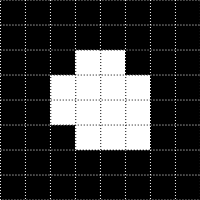
\includegraphics{ref_marker_grid.png}

    
\end{center}
    \item Here the 1 represent white colour and 0 represents black colour.
\end{enumerate}


\subsection{Finding the Orientation and Binary Value}
\begin{enumerate}
    \item Once we have the 8x8 matrix, we try to find the position of the white box present in the corner of the
4x4 matrix, which will give us the orientation of the tag.
    \item The position of the white box determines how much has the tag been rotated.
    \item  Once we have the angle of rotation we find the value of tag ID through the 2x2 matrix in between.
    \item  We get the tag in the actual rotation and check the inner 2x2 value for zeros and ones.
\end{enumerate}
\begin{center}

    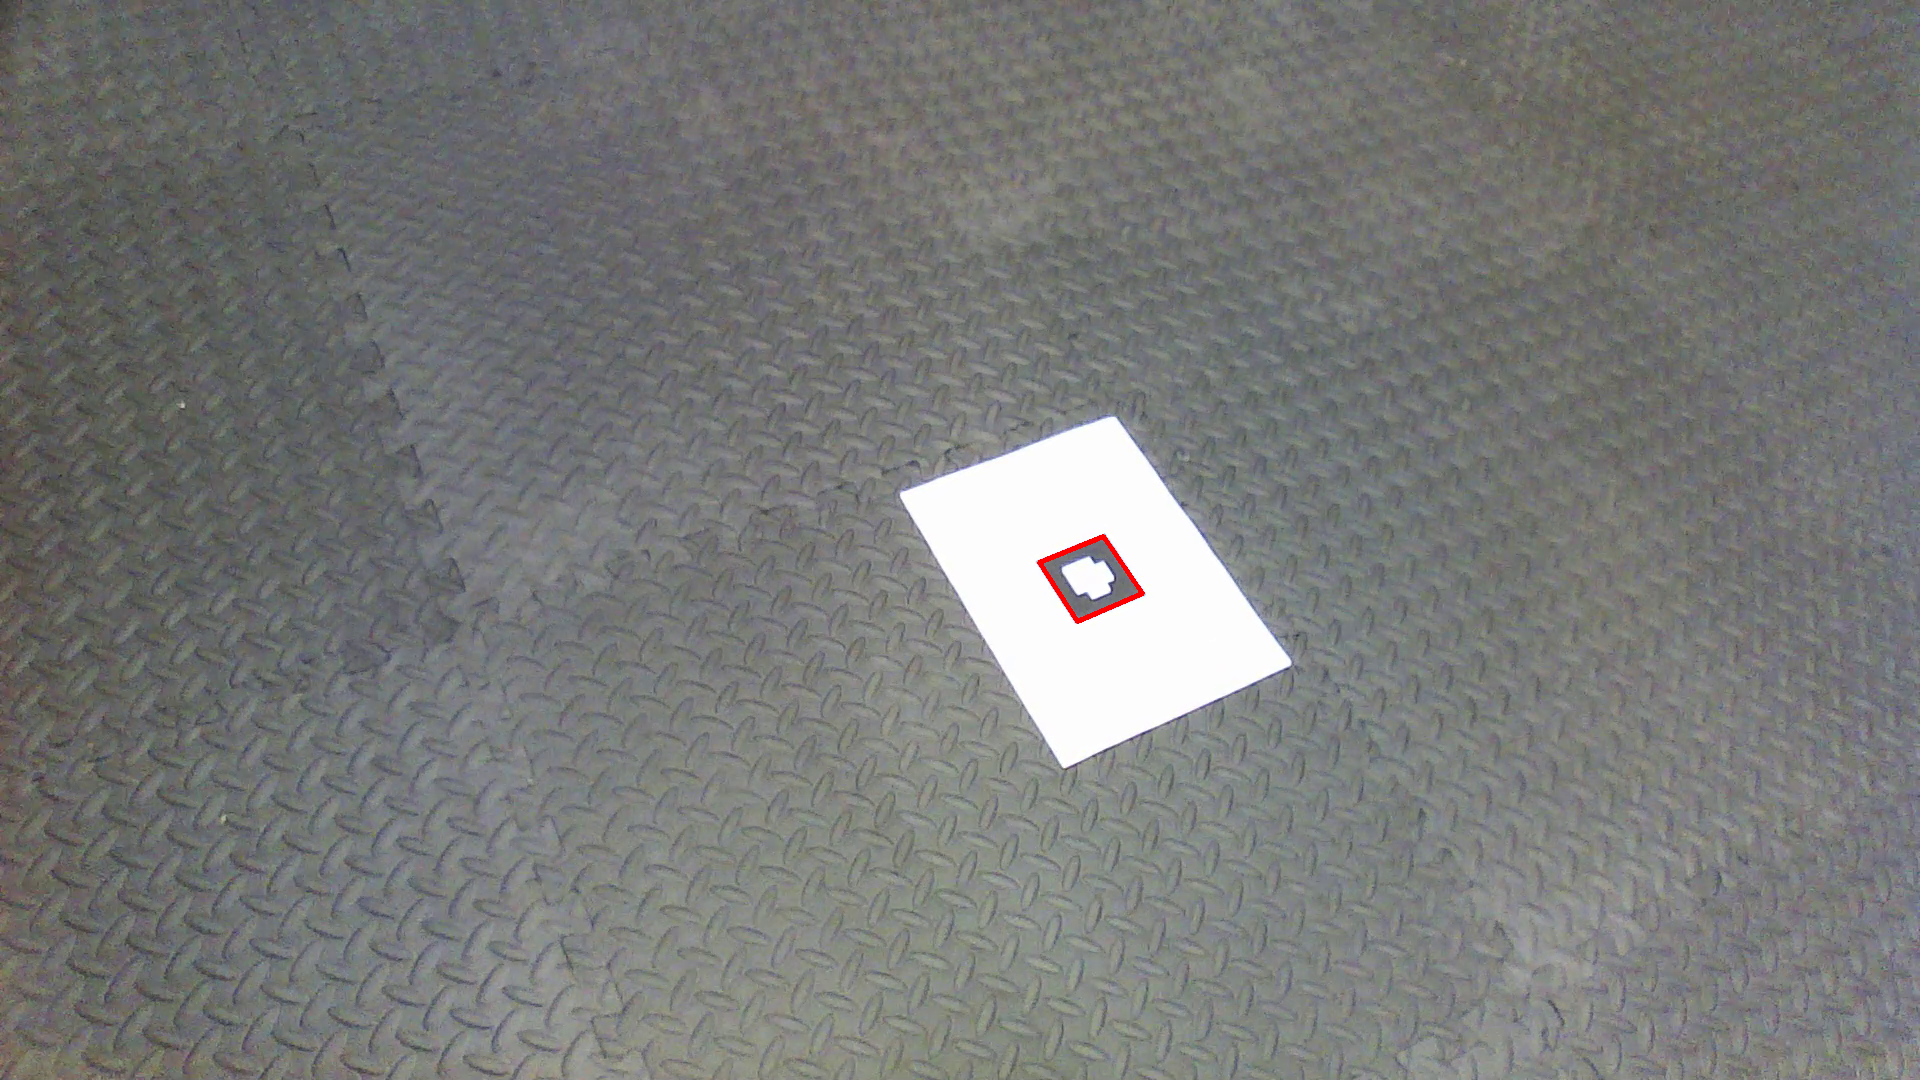
\includegraphics[scale=0.2]{tag detection.png}

    
\end{center}
\section{Problem 2}

\subsection{Superimposing an image onto the tag}
\begin{enumerate}
    \item  The corners of the AR tag in the videos from section-2 are used in this section.
    \item  The corners are updated according to the orientation of the AR-Tag.
    \item  The image of Lena is to be superimposed onto the AR tag
    \begin{center}

    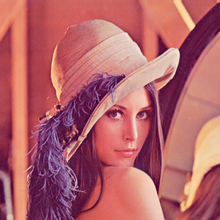
\includegraphics{220px-Lenna_(test_image).png}

    
\end{center}
    \item A homography function is defined to estimate the homographic matrix,H between the given template,
image of Lena(world frame) and the coordinates of the corners of the AR tags(camera frame), based
on the relations and equations provided in the supplementary reading file.
    \item Using inverse homography the camera frame coordinates corresponding to the world frame could be
obtained.Therefore by applying inverse homography to each pixel of the template, the corresponding pixel
of the camera frame could be determined.
    \item After finding the relation between the camera frame and world frame, the pixels of camera frame are
simply replaced by the corresponding pixels of the world frame
    \item The orientation of the image/template matches to that of the AR tag which is clearly observed in the
video since there is no flip or disorientation of the image with the changing orientation of the camera.
\end{enumerate}
\begin{center}

    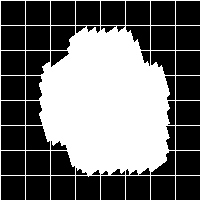
\includegraphics[scale=0.5]{perspectiveProjection.png}
    \includegraphics[scale=0.25]{Lena1.png}
    \includegraphics[scale=0.25]{Lena2.png}
    \includegraphics[scale=0.25]{Lena3.png}
    \includegraphics[scale=0.25]{Lena4.png}
    

\end{center}
\subsection{Placing a virtual cube on the tag}
Augmented reality applications generally place 3D objects onto the real world, which maintain the three
dimensional properties such as rotation and scaling as you move around the “object” with your camera. In
this part of the project you will implement a simple version of the same, by placing a 3D cube on the tag.
This is the process of “projecting” a 3D shape onto a 2D image.

\begin{enumerate}
    \item The homography between the world coordinates (the reference AR tag) and the image plane (the tag in the image sequence) is first computed. The calculation of this has been done by detecting the four corners of the marker in the input image captured by camera i.e the true corners for the UPRIGHT orientation of marker).
    \item The world coordinates of the corners is determined and the homography is computed between the detected corner points in the image (pixel coordinates) and the corresponding points in the reference (world) coordinate system.
    \item The projection matrix is then built from the given camera calibration matrix provided and the homog- raphy matrix. Here the camera’s pose i.e the rotation matrix R and translation vector t is found as shown in the code, and thus the projection matrix, P = K[R|t] is constructed.
    \item Assuming that the virtual cube is sitting on “top” of the marker, and that the Z axis is negative in the upwards direction, we have obtained the coordinates of the other four corners of the cube. This allows the transformation of all the corners of the cube onto the image plane using the projection matrix.
    \item The formulas and equations required for defining the homography and projectionMatrix functions are
referred from the supplementary provided.
    \item The cube is then drawn using cv2.drawContours
\end{enumerate}
\begin{center}

    \includegraphics[scale=0.25]{cube1.png}
    \includegraphics[scale=0.25]{cube2.png}
    \includegraphics[scale=0.25]{cube3.png}
    \includegraphics[scale=0.25]{cube4.png}
    

    
\end{center}
\section{Problems Encountered}
\begin{enumerate}
    \item For the corner detection of the AR tag first we were trying to use Harris corner and goodfeaturestotrack algorithm but the problem was that the corner points output which these were returning are randomly organised so it was difficult to separate and say to which contours they belong,as there can be contour of the white paper and other unwanted detection's are possible.So we used cv2.findContours from which the unwanted contour can be discarded using the hierarchy of contours which this function returns
    
    \item For implementing warping we initially using two for loops which were computationally intensive and time consuming,so we had to come up with the vectorised implementation of warping function
 
\end{enumerate}




\end{document}